\documentclass[14pt]{beamer}

\usetheme[secheader]{Boadilla}

% Presento style file
\usepackage{tikz}
\usetikzlibrary{tikzmark,fit,shapes.geometric}

% Information
\title{Courbes planes paramétrées}
\subtitle{Partie 2}
\author{Y. Carissan}
%\institute{www.ratulsaha.com}
\date{2020}

\AtBeginSection[]{\begin{frame}{Plan}\tableofcontents[currentsection,hideothersubsections]\end{frame}}

\begin{document}

% Title page
\begin{frame}{}
\maketitle
\end{frame}

\begin{frame}{Plan}
        \tableofcontents[hideallsubsections]
\end{frame}

\section{Courbes planes en paramétrage polaire}
\subsection{Coordonnées polaires}
\begin{frame}{Coordonnées polaires}
        \begin{alertblock}{Définition~:}
                Soit un point du plan $M$ tel que $M\ne O$.\\
                Soit $\vec{u}$ un vecteur directeur unitaire de $\vec{OM}$.\\
                On appelle coordonnées polaires de $M$ le couple $(\theta;r)$
                tels que~:
                \begin{align*}
                        \left\{\begin{array}{l}
                                \theta = \widehat{(\vec{i}, \vec{u})}\\
                                \vec{OM} = r\vec{u}
                        \end{array}\right.
                \end{align*}
        \end{alertblock}
\end{frame}
\begin{frame}
        \begin{block}{Méthode}
                On place successivement~:
                \begin{enumerate}
                                \item<1-> $\theta$
                                \item<2-> $\vec{u}$ grâce à la formule $\theta = \widehat{(\vec{i}, \vec{u})}$
                                \item<3-> $M$ grâce à la formule $\vec{OM} = r\vec{u}$
                \end{enumerate}
                \begin{center}
                        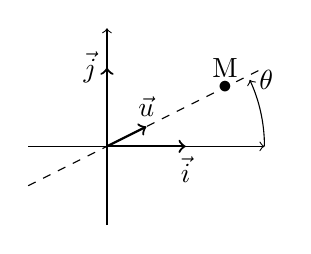
\begin{tikzpicture}
                                \draw[->] (-1,0) -- (2,0);
                                \draw[->] (0,-1.0) -- (0,1.5);
                                \onslide<1>{\draw[->,thick] (0,0) -- (1,0) node [below] {$\vec{i}$};
                                \draw[->,thick] (0,0) -- (0,1) node [left] {$\vec{j}$};}
                                \draw[dashed] (-1,-0.5) -- (2,1);
                                \onslide<1>{\draw[->] (2,0) arc(0:25:2) node [right] {$\theta$};}
                                \onslide<2>{\draw[->,thick] (0,0) -- (0.5,0.25) node [above] {$\vec{u}$};}
                                \onslide<3>{\draw (1.5,0.75) node {$\bullet$} node [above] {M};}
                        \end{tikzpicture}
                \end{center}
        \end{block}
        \onslide<3>{%
        \begin{alertblock}{Attention}
                $r\in\mathbb{R}$ donc $r$ peut être positif ou négatif.
        \end{alertblock}
        }
\end{frame}
\begin{frame}
        \begin{block}{Remarques}
                \begin{enumerate}
                                \item Les coordonnées polaires d'un point ne sont pas uniques:
                                        $(\theta;r)$, $(\theta+2k\pi;r)$ et $(\theta+\pi+2k\pi;-r)$
                                        sont les coordonnées du même point;
                                \item $O$ n'a pas de coordonnées polaires, on lui ajouter les coordonnées
                                        $(\theta; r=0)$, la valeur de $\theta$ sera donnée par
                                        la courbe.
                \end{enumerate}
        \end{block}
\end{frame}
\subsection{Passage cartésiennes $\leftrightarrow$ polaires}
\begin{frame}{Passage cartésiennes $\leftrightarrow$ polaires}
        \begin{alertblock}{Proposition}
                Soit $(x;y)$ les coordonnées cartésiennes de $M$.\\
                Soit $(\theta;r)$ les coordonnées polaires de $M$.\\
                Alors~:
                \begin{align*}
                        \left\{\begin{array}{l}
x=r\cos \theta\\
y=r\sin \theta
                        \end{array}\right. & \Leftrightarrow
                        \left\{\begin{array}{l}
                                r=\epsilon\sqrt{x^2 + y^2}\\
                                \cos\theta=\frac{x}{\epsilon\sqrt{x^2 + y^2}}\\
                                \sin\theta=\frac{y}{\epsilon\sqrt{x^2 + y^2}}
                        \end{array}\right.
                        \text{avec }\epsilon\in\left\{-1;+1\right\}
                \end{align*}
        \end{alertblock}
\end{frame}
\subsection{Courbes classiques}
\subsubsection{Droite passant par l'origine}
\begin{frame}{Droite passant par l'origine}
        \begin{alertblock}{Droite passant par $O$ de pente $\alpha$}
                Soit $(D)$ une droite passant par $O$.\\
                $(D)$ a pour équation $\theta=\alpha$.\\
                \begin{center}
                        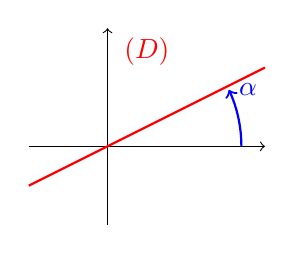
\begin{tikzpicture}
                                \draw[->] (-1,0) -- (2,0);
                                \draw[->] (0,-1.0) -- (0,1.5);
                                \draw[color=red, thick] (-1,-0.5) -- (2,1);
                                \draw[red] (0.5,1.2) node {$(D)$};
                                \onslide<1>{\draw[->,thick,color=blue] (1.7,0) arc(0:25:1.7) node [right] {$\alpha$};}
                \end{tikzpicture}
                \end{center}
        \end{alertblock}
\end{frame}

\subsubsection{Droite ne passant pas par l'origine}
\begin{frame}{Droite ne passant pas par l'origine}
        \begin{alertblock}{Droite ne passant par $O$}
                Soit $(D)$ une droite ne passant pas par $O$.\\
                $(D)$ a pour équation polaire~:
                \begin{align*}
                        r=\frac{1}{\lambda\cos\theta+\mu\sin\theta}
                \end{align*}
                où $\lambda$ et $\mu$ sont deux constantes réelles.
        \end{alertblock}
\end{frame}
\begin{frame}{Droite ne passant pas par l'origine}
        \begin{exampleblock}{Exemple d'une droite ne passant par $O$}
                Soit la droite telle que $\lambda=2$ et $\mu=1$.\\
                \begin{minipage}[c]{0.4\textwidth}
                \begin{tabular}{c|l|r}
                        Point & $\theta$ & $r$ \\\hline
                        A & $0$              & $0.500$  \\
                        B & $\frac{\pi}{8}$  & $0.448$  \\
                        C & $\frac{2\pi}{8}$ & $0.471$  \\
                        D & $\frac{3\pi}{8}$ & $0.592$  \\
                        E & $\frac{4\pi}{8}$ & $1.000$  \\
                        F & $\frac{5\pi}{8}$ & $6.309$  \\
                        G & $\frac{6\pi}{8}$ & $-1.414$ \\
                        H & $\frac{7\pi}{8}$ & $-0.683$ \\
                \end{tabular}
                \end{minipage}
                \hfill
                \begin{minipage}[c]{0.4\textwidth}
                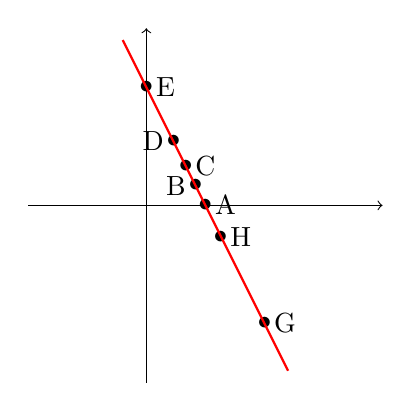
\begin{tikzpicture}[scale=1.5]
                        \draw[->] (-1,0) -- (2,0);
                        \draw[->] (0,-1.5) -- (0,1.5);
                        \draw ( 0.0: 0.5           ) node {$\bullet$} node [right] {A};
                        \draw (  22:0.448341529168 ) node {$\bullet$} node [left] {B};
                        \draw (  45:0.471404520791 ) node {$\bullet$} node [right] {C};
                        \draw (  67:0.591979951316 ) node {$\bullet$} node [left] {D};
                        \draw (  90:1.0            ) node {$\bullet$} node [right] {E};
%                        \draw ( 112:6.3086440598   ) node {$\bullet$} node [right] {F};
                        \draw ( 135:-1.41421356237 ) node {$\bullet$} node [right] {G};
                        \draw ( 157:-0.68255861862 ) node {$\bullet$} node [right] {H};
                        \draw [thick, red] ( -0.2, 1.4) -- ( 1.2, -1.4);
                \end{tikzpicture}
                \end{minipage}\\
                Le point F, pour $\theta=\frac{5\pi}{8}$, n'est pas représenté.
        \end{exampleblock}
\end{frame}
\subsubsection{Cercle de centre l'origine du repère}
\begin{frame}{Cercle de centre l'origine du repère}
        \begin{alertblock}{Proposition}
                Le cercle de centre $O$ et de rayon R a pour équation $r=R$.
        \end{alertblock}
\end{frame}
\subsubsection{Cercle passant par l'origine du repère}
\begin{frame}{Cercle passant par l'origine du repère}
        \begin{alertblock}{Proposition}
                Les cercles qui passent par $O$
                ont pour équation polaire~:
                \begin{align*}
                        r=\lambda\cos\theta+\mu\sin\theta
                \end{align*}
                où $\lambda$ et $\mu$ désignent deux constantes réelles.
        \end{alertblock}
\end{frame}

\subsection{Tangente en un point}
\subsubsection{Tangente en un point distinct de l'origine}
\begin{frame}{Tangente en un point distinct de l'origine}
        \begin{alertblock}{Proposition}
                Soit $(\mathcal{C})$ une courbe d'équation polaire $r=f(\theta)$.\\
                Soit $M$ un point de $(\mathcal{C})$, distinct de l'originie.\\
                Alors la tangente en $M$ est dirigée par $\vec{OM\;'}(\theta)$.
        \end{alertblock}
\end{frame}
\begin{frame}{Tangente en un point distinct de l'origine}
        \begin{block}{Preuve}
                \begin{itemize}
                                \item<1-> On sait que la tangente est dirigée par le premier
                                        vecteur dérivé non nul.\\
                                        \only<1>{\alert{On cherche donc si $\vec{OM\;'}(\theta)\ne 0$}}
                                \item<2-> \only<2>{On pose $\vec{OM}(\theta) = r(\theta)\vec{u}(\theta)$\\
                                        Donc }$\vec{OM\;'}(\theta) = r\;'(\theta)\vec{u}(\theta)
                                        +r(\theta)\vec{u\;'}(\theta)$.
                                \item<3-> \only<3>{Or $\vec{u}(\theta)=\left|\begin{array}{l}\cos\theta\\\sin\theta\end{array}\right.$
                                                et $\vec{u\;'}(\theta)=\left|\begin{array}{l}-\sin\theta\\\cos\theta\end{array}\right.$.\\
                                                        $\vec{u}(\theta).\vec{u\;'}(\theta)=-\cos\theta\sin\theta+\sin\theta\cos\theta=0$\\
                                      Donc }$\vec{u}(\theta)\perp\vec{u\;'}(\theta)$.\\
                                      \only<3>{\alert{Donc toute combinaison linéaire de $\vec{u}$ et $\vec{u\;'}$ sera
                                      non nulle.}}
                                \item<4-> De plus, comme $M\ne O$ alors $r(\theta)\ne 0$.
                                \item<5-> On en déduit que $\vec{OM\;'}(\theta)\ne\vec{0}$, donc
                                        la tangente en $M$ est dirigée par $\vec{OM\;'}(\theta)$.

                \end{itemize}
        \end{block}
\end{frame}
\begin{frame}{}
        \begin{block}{Remarque}
                On retiendra que les vecteurs $\vec{u}(\theta)$ et $\vec{u\;'}(\theta)$
                sont positivement orthogonaux. Cela signifie que~:
                \begin{enumerate}
                                \item $\vec{u}(\theta)\perp\vec{u\;'}(\theta)$
                                \item $\widehat{\left(\vec{u}(\theta);\vec{u\;'}(\theta)\right)}=+\frac{\pi}{2}\;[2\pi]$
                \end{enumerate}
                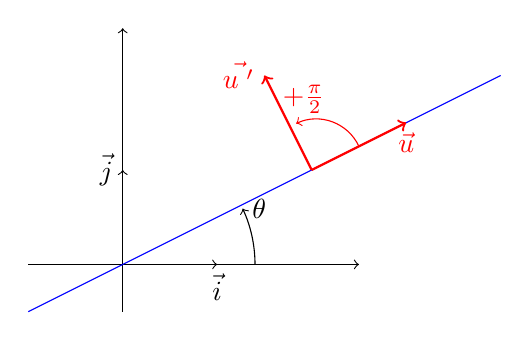
\begin{tikzpicture}[scale=1.2]
                        \draw[->] (-1,0) -- (2.5,0);
                        \draw[->] (0,-0.5) -- (0,2.5);
                        \draw[->] (0,0) -- (1,0) node [below] {$\vec{i}$};
                        \draw[->] (0,0) -- (0,1) node [left] {$\vec{j}$};
                        \draw[blue] (-1.0,-0.50) -- (4,2.0);
                        \draw[->] (1.4,0) arc(0:25:1.4) node [right] {$\theta$};
                        \draw[->,red,thick] (2,1) -- (3,1.5) node [below] {$\vec{u}$};
                        \draw[->,red,thick] (2,1) -- (1.5,2) node [left] {$\vec{u\;'}$};
                        \draw[->,red] (2.5,1.25) arc(25:115:0.5) node [above] {$\;\;+\frac{\pi}{2}$};
                \end{tikzpicture}
        \end{block}
\end{frame}
\end{document}
